%%%%%%%%%%%%%%%%%%%%%%%%%%%%%%%%%%%%%%%%%
% Diaz Essay
% LaTeX Template
% Version 2.0 (13/1/19)
%
% This template originates from:
% http://www.LaTeXTemplates.com
%
% Authors:
% Vel (vel@LaTeXTemplates.com)
% Nicolas Diaz (nsdiaz@uc.cl)
%
% License:
% CC BY-NC-SA 3.0 (http://creativecommons.org/licenses/by-nc-sa/3.0/)
%
%%%%%%%%%%%%%%%%%%%%%%%%%%%%%%%%%%%%%%%%%

%----------------------------------------------------------------------------------------
%	PACKAGES AND OTHER DOCUMENT CONFIGURATIONS
%----------------------------------------------------------------------------------------

\documentclass[12pt]{diazessay} % Font size (can be 10pt, 11pt or 12pt)

%----------------------------------------------------------------------------------------
%	TITLE SECTION
%----------------------------------------------------------------------------------------

\title{\textbf{Course: Física Teórica I (CDP7600)} \\[0.2cm] {\Large \textbf{Project}: \hspace{0.2cm}
\textit{Fibration building blocks of information-processing networks}
}}% Title and subtitle

\author{\textbf{Higor da S. Monteiro} \\ \textit{Universidade Federal do Ceará}} % Author and institution

\date{\today} % Date, use \date{} for no date

%----------------------------------------------------------------------------------------

\begin{document}

\maketitle % Print the title section

%----------------------------------------------------------------------------------------
%	ABSTRACT AND KEYWORDS
%----------------------------------------------------------------------------------------

%\renewcommand{\abstractname}{Summary} % Uncomment to change the name of the abstract to something else

\begin{abstract}
	Fibration building blocks of a network represent the sets of nodes that are symmetric with respect to information processing. Here, we have reproduced important results concerning the identification and classification of the fibration building blocks of directed networks, constructed from real network data. More specifically, using the transcriptional regulatory network data of the \textit{Escherichia Coli} bacteria, we quantify the groups of network nodes that synchronously process equivalent information and then we classify each fiber based on its specific topological features. This way, in order to consistently present the obtained results, in this report we first give a brief description of the theory concerning the graph fibration morphism and its main definitions related to information flow symmetries. Next, we detail the methods adopted to correctly identify and classify the network fibers. More specifically, to establish an optimal framework, I show the implementation details of the Minimal Balanced Coloring algorithm used to find the corresponding fibers in the network, presenting a slightly improvement for the algorithm complexity. At last, showing the proper methods for data preparation, I describe the results obtained concerning the fiber statistics for the specific case of the \textit{Escherichia Coli} regulatory network, to properly compare with the recent results presented at \textit{Morone et. al.} (2019).
\end{abstract}

\hspace*{3.6mm}\textit{Keywords:} Graph Morphism; Biological Networks; Information Processing, Fibration, lectus % Keywords

\vspace{30pt} % Vertical whitespace between the abstract and first section

%----------------------------------------------------------------------------------------
%	ESSAY BODY
%----------------------------------------------------------------------------------------

\section{Brief Introduction}

This statement requires citation \cite{fibration2019}; this one does too \cite{Cardon1982} \cite{Boldi2006} \cite{Tarjan1987} \cite{Stewart2006}. Lorem ipsum dolor sit amet, consectetur adipiscing elit. Aenean dictum lacus sem, ut varius ante dignissim ac. Sed a mi quis lectus feugiat aliquam. Nunc sed vulputate velit. Sed commodo metus vel felis semper, quis rutrum odio vulputate. Donec a elit porttitor, facilisis nisl sit amet, dignissim arcu. Vivamus accumsan pellentesque nulla at euismod. Duis porta rutrum sem, eu facilisis mi varius sed. Suspendisse potenti. Mauris rhoncus neque nisi, ut laoreet augue pretium luctus. Vestibulum sit amet luctus sem, luctus ultrices leo. Aenean vitae sem leo.

\begin{figure}[h]
	\centering
	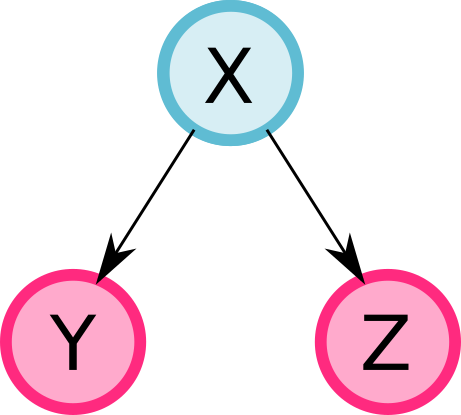
\includegraphics[scale=0.4]{Figures/ex1.png}
\end{figure}
\begin{figure}[h]
	\centering
	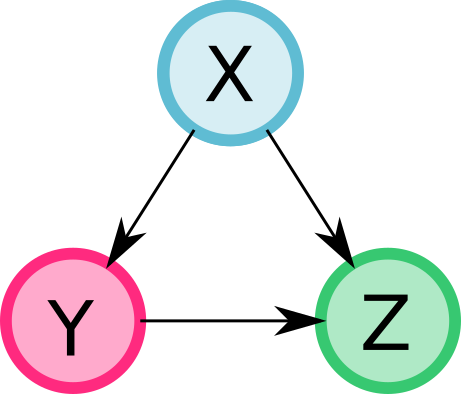
\includegraphics[scale=0.4]{Figures/ex2.png}
\end{figure}

Nullam semper quam at ante convallis posuere. Ut faucibus tellus ac massa luctus consectetur. Nulla pellentesque tortor et aliquam vehicula. Maecenas imperdiet euismod enim ut pharetra. Suspendisse pulvinar sapien vitae placerat pellentesque. Nulla facilisi. Aenean vitae nunc venenatis, vehicula neque in, congue ligula.

Pellentesque quis neque fringilla, varius ligula quis, malesuada dolor. Aenean malesuada urna porta, condimentum nisl sed, scelerisque nisi. Suspendisse ac orci quis massa porta dignissim. Morbi sollicitudin, felis eget tristique laoreet, ante lacus pretium lacus, nec ornare sem lorem a velit. Pellentesque eu erat congue, ullamcorper ante ut, tristique turpis. Nam sodales mi sed nisl tincidunt vestibulum. Interdum et malesuada fames ac ante ipsum primis in faucibus.

\begin{figure}[h]
	\centering
	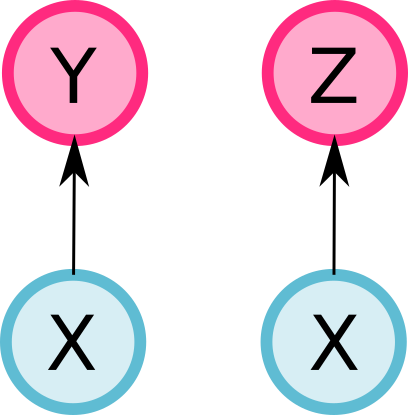
\includegraphics[scale=0.4]{Figures/ex1input.png}
\end{figure}
\begin{figure}[h]
	\centering
	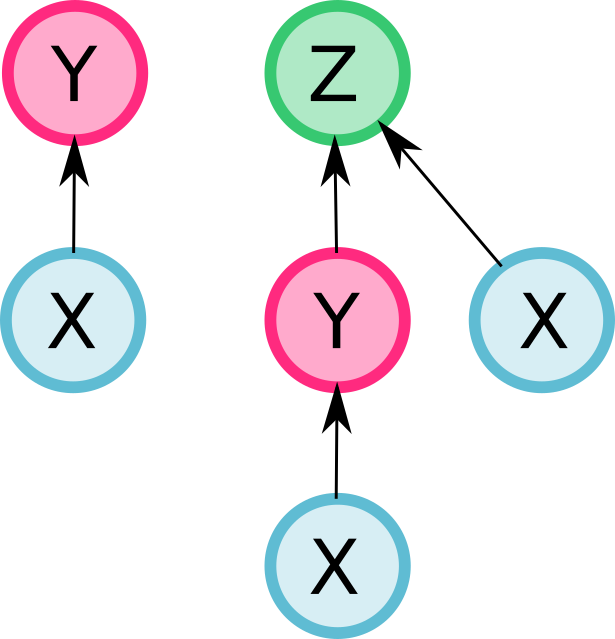
\includegraphics[scale=0.4]{Figures/ex2input.png}
\end{figure}

%------------------------------------------------

\section{\textit{Minimal Balanced Coloring }Algorithm}

\subsection{Algorithm description}

For the proper identification of the fibers on the network we have to construct a graph partition that is equivalent to a coarse grain of the network with respect to the information flow passing through each node.

Aliquam fringilla non diam sed varius. Suspendisse tellus felis, hendrerit non bibendum ut, adipiscing vitae diam. Lorem ipsum dolor sit amet, consectetur adipiscing elit. Nulla lobortis purus eget nisl scelerisque, commodo rhoncus lacus porta. Vestibulum vitae turpis tincidunt, varius dolor in, dictum lectus. Aenean ac ornare augue, ac facilisis purus. Sed leo lorem, molestie sit amet fermentum id, suscipit ut sem. Vestibulum orci arcu, vehicula sed tortor id, ornare dapibus lorem. Praesent aliquet iaculis lacus nec fermentum. Morbi eleifend blandit dolor, pharetra hendrerit neque ornare vel. Nulla ornare, nisl eget imperdiet ornare, libero enim interdum mi, ut lobortis quam velit bibendum nibh.

\begin{itemize}
	\item First bullet point item
	\item Second bullet point item
	\item Third bullet point item
\end{itemize}

\subsection{Data preparation and algorithm implementation}

Morbi tempor congue porta. Proin semper, leo vitae faucibus dictum, metus mauris lacinia lorem, ac congue leo felis eu turpis. Sed nec nunc pellentesque, gravida eros at, porttitor ipsum. Praesent consequat urna a lacus lobortis ultrices eget ac metus. In tempus hendrerit rhoncus. Mauris dignissim turpis id sollicitudin lacinia. Praesent libero tellus, fringilla nec ullamcorper at, ultrices id nulla. Phasellus placerat a tellus a malesuada.

\begin{enumerate}
	\item First numbered list item
	\item Second numbered list item
\end{enumerate}

%------------------------------------------------

\section*{Results}

Fusce in nibh augue. Cum sociis natoque penatibus et magnis dis parturient montes, nascetur ridiculus mus. In dictum accumsan sapien, ut hendrerit nisi. Phasellus ut nulla mauris. Phasellus sagittis nec odio sed posuere. Vestibulum porttitor dolor quis suscipit bibendum. Mauris risus lectus, cursus vitae hendrerit posuere, congue ac est. Suspendisse commodo eu eros non cursus. Mauris ultrices venenatis dolor, sed aliquet odio tempor pellentesque. Duis ultricies, mauris id lobortis vulputate, tellus turpis eleifend elit, in gravida leo tortor ultricies est. Maecenas vitae ipsum at dui sodales condimentum a quis dui. Nam mi sapien, lobortis ac blandit eget, dignissim quis nunc.

Donec luctus tincidunt mauris, non ultrices ligula aliquam id. Sed varius, magna a faucibus congue, arcu tellus pellentesque nisl, vel laoreet magna eros et magna. Vivamus lobortis elit eu dignissim ultrices. Fusce erat nulla, ornare at dolor quis, rhoncus venenatis velit. Donec sed elit mi. Sed semper tellus a convallis viverra. Maecenas mi lorem, placerat sit amet sem quis, adipiscing tincidunt turpis. Cras a urna et tellus dictum eleifend. Fusce dignissim lectus risus, in bibendum tortor lacinia interdum.

\begin{table}[h] % [h] forces the table to be output where it is defined in the code (it suppresses floating)
	\caption{Example table.}
	\centering
	\begin{tabular}{l l r}
		\toprule
		\multicolumn{2}{c}{Name} \\
		\cmidrule(r){1-2}
		First Name & Last Name & Grade \\
		\midrule
		John & Doe & $7.5$ \\
		Richard & Miles & $5$ \\
		\bottomrule
	\end{tabular}
\end{table}

Fusce eleifend porttitor arcu, id accumsan elit pharetra eget. Mauris luctus velit sit amet est sodales rhoncus. Donec cursus suscipit justo, sed tristique ipsum fermentum nec. Ut tortor ex, ullamcorper varius congue in, efficitur a tellus. Vivamus ut rutrum nisi. Phasellus sit amet enim efficitur, aliquam nulla id, lacinia mauris. Quisque viverra libero ac magna maximus efficitur. Interdum et malesuada fames ac ante ipsum primis in faucibus. Vestibulum mollis eros in tellus fermentum, vitae tristique justo finibus. Sed quis vehicula nibh. Etiam nulla justo, pellentesque id sapien at, semper aliquam arcu. Integer at commodo arcu. Quisque dapibus ut lacus eget vulputate.

\section{Conclusion}

Nullam semper quam at ante convallis posuere. Ut faucibus tellus ac massa luctus consectetur. Nulla pellentesque tortor et aliquam vehicula. Maecenas imperdiet euismod enim ut pharetra. Suspendisse pulvinar sapien vitae placerat pellentesque. Nulla facilisi. Aenean vitae nunc venenatis, vehicula neque in, congue ligula.


%----------------------------------------------------------------------------------------
%	BIBLIOGRAPHY
%----------------------------------------------------------------------------------------

\bibliographystyle{unsrt}

\bibliography{sample.bib}

%----------------------------------------------------------------------------------------

\end{document}
